% Currículo de João Gabriel Salvador Paiva — perfil Mobile (Flutter/Dart), versão em português
% Genérico para vagas de Desenvolvedor Mobile Flutter pleno.
% Layout de coluna única, texto 100% selecionável, sem tabelas nem caixas de texto (ATS-friendly).
\documentclass[10.5pt,a4paper]{article}

\usepackage[T1]{fontenc}
\usepackage[utf8]{inputenc}
\usepackage[brazil]{babel}
\usepackage{lmodern}
\usepackage[margin=1.5cm,top=1.2cm,bottom=1.2cm]{geometry}
\usepackage{graphicx}
\usepackage{enumitem}
\usepackage{titlesec}
\usepackage{xcolor}
\usepackage[hidelinks]{hyperref}
\usepackage{microtype}
\usepackage{needspace}

\definecolor{azul}{HTML}{14375A}

\hypersetup{
  pdftitle={Joao Gabriel Salvador Paiva - Desenvolvedor Mobile Flutter},
  pdfauthor={Joao Gabriel Salvador Paiva},
  pdfsubject={Curriculo - Desenvolvedor Mobile Flutter},
  pdfkeywords={Flutter, Dart, mobile, Android, iOS, App Store, Google Play, BLoC, gerenciamento de
  estado, testes unitarios, widget tests, testes de integracao, API REST, FastAPI, Python, Git,
  CI/CD, GitHub Actions, Clean Code, SOLID, Scrum}
}

\pagestyle{empty}
\setlength{\parindent}{0pt}
\setlength{\emergencystretch}{2em}
\setlist[itemize]{leftmargin=3.6mm,itemsep=1pt,topsep=2pt,parsep=0pt,label=\textbullet}

\titleformat{\section}{\bfseries\large\color{azul}}{}{0em}{}[\vspace{-1.2ex}\rule{\linewidth}{0.6pt}]
\titlespacing{\section}{0pt}{2.2ex}{1.2ex}

\newcommand{\cargo}[4]{%
  \Needspace*{5\baselineskip}%
  \textbf{#1} \textnormal{---} #2 \hfill \textnormal{#3}\\
  \textit{\small #4}\vspace{0.4ex}
}

\begin{document}

%% ---------- Cabeçalho ----------
\begin{minipage}[c]{0.78\textwidth}
\raggedright
{\LARGE\bfseries\color{azul} João Gabriel Salvador Paiva}\\[0.6ex]
{\large Desenvolvedor Mobile --- Flutter \& Dart}\\[0.9ex]
\small
Campina Grande – PB, Brasil (disponível para trabalho remoto)\\
\href{mailto:joaogabrielsalvadorpaiva@gmail.com}{joaogabrielsalvadorpaiva@gmail.com} $\cdot$ +55 (83) 98863-6734\\
\href{https://github.com/Ilusinusmate}{github.com/Ilusinusmate} $\cdot$
\href{https://www.linkedin.com/in/joao-gabriel-salvador-paiva-805283286}{linkedin.com/in/joao-gabriel-salvador-paiva} $\cdot$
\href{https://ilusinusmate.github.io/Ilusinusmate/}{ilusinusmate.github.io/Ilusinusmate}
\end{minipage}\hfill
\begin{minipage}[c]{0.2\textwidth}
\raggedleft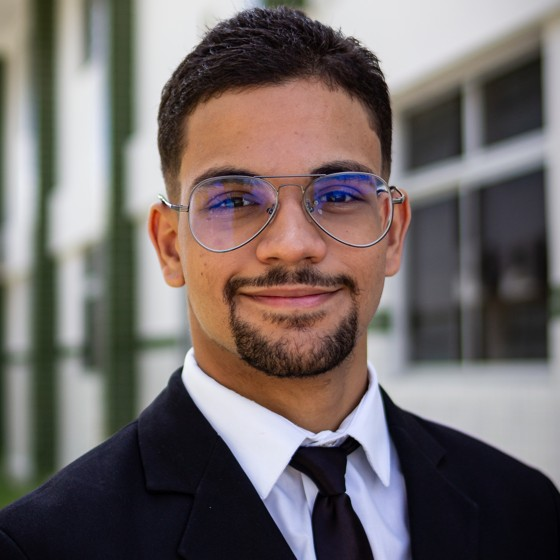
\includegraphics[width=2.7cm]{foto.jpg}
\end{minipage}

%% ---------- Resumo ----------
\section*{Resumo}
Desenvolvedor mobile responsável pelo aplicativo \textbf{Central da Escola} (\textbf{Flutter/Dart}),
com mais de \textbf{50 mil usuários ativos}, do qual sou o único desenvolvedor desde a versão 3 e
onde lidero o setor de desenvolvimento mobile. Cubro o ciclo completo do produto: implementação de
funcionalidades, \textbf{testes}, \textbf{CI/CD}, \textbf{publicação nas lojas Android e iOS},
monitoramento em produção e evolução contínua. Também desenvolvo o \textbf{backend} que sustenta o
app (\textbf{Python/FastAPI}, \textbf{APIs REST}, microsserviços e mensageria), o que me permite
integrar aplicativo e serviços de ponta a ponta. Graduando em Ciência da Computação na UFCG e
residente em TIC no VIRTUS-CC/UFCG.

%% ---------- Competências ----------
\section*{Competências técnicas}
\textbf{Mobile:} Flutter, Dart, Android, iOS, publicação na Google Play e na App Store,
gerenciamento de estado (BLoC), componentização, \textit{context isolation}, ciclo de release e
monitoramento em produção\\
\textbf{Qualidade mobile:} testes automatizados, code review,
Clean Code, SOLID, DRY, design patterns, arquitetura em camadas\\
\textbf{Integrações:} APIs REST, WebSocket, autenticação, integrações com sistemas internos e de
terceiros\\
\textbf{Backend (complementar):} Python, FastAPI, Django, microsserviços, PostgreSQL, NoSQL, Redis,
RabbitMQ, MinIO\\
\textbf{Engenharia:} Git (\textit{feature branches} e \textit{pull requests}), GitHub Actions,
CI/CD, Docker, AWS, logging e observabilidade (OpenTelemetry, Grafana), documentação técnica,
Scrum/Kanban

%% ---------- Experiência ----------
\section*{Experiência profissional}

\cargo{Logon Informática}{Mobile \& Backend Developer}{jan/2025 -- atual}{Software house de
sistemas de gestão para educação, administração pública e outros setores}
\begin{itemize}
  \item Único desenvolvedor do aplicativo \textit{Central da Escola} desde a \textbf{versão 3}, em
        \textbf{Flutter/Dart}, com mais de \textbf{50 mil usuários ativos} em Android e iOS.
  \item \textbf{Lidero o setor de desenvolvimento mobile}: definição de funcionalidades,
        priorização, code review e documentação técnica do time.
  \item Conduzo o \textbf{ciclo completo de release}: desenvolvimento, testes, \textbf{CI/CD} e
        \textbf{publicação nas lojas Google Play e App Store}, com logging e acompanhamento do app
        em produção.
  \item Desenvolvo os \textbf{microsserviços em Python/FastAPI} consumidos pelo app, com
        \textbf{APIs REST}, comunicação assíncrona via \textbf{RabbitMQ} e armazenamento de objetos
        em \textbf{MinIO}.
  \item Atuo como ponto de \textbf{mediação entre times} (produto, backend e áreas internas) para
        integrações internas e com sistemas de terceiros.
  \item Publiquei o \textbf{pdfa-parser} no PyPI, biblioteca open source de conversão e validação de
        PDF/A usada como apoio aos produtos da empresa.
\end{itemize}

\cargo{Empório Sertanejo}{Desenvolvedor Full-stack --- líder técnico}{dez/2023 -- set/2025}{Franquia
de varejo; SaaS proprietário de ERP, PDV e e-commerce}
\begin{itemize}
  \item \textbf{Liderei 3 desenvolvedores} na construção de um SaaS que unificou \textbf{ERP, PDV e
        e-commerce}, em \textbf{Django/Python} com \textbf{PostgreSQL} e \textbf{Docker}.
  \item Implantei \textbf{testes automatizados} (PyTest e mocks), \textbf{CI/CD com GitHub Actions}
        e \textbf{observabilidade} (OpenTelemetry e Grafana) para investigar erros em homologação e
        produção.
  \item Conduzi levantamento de requisitos e negociação diretamente com o cliente por mais de
        2 anos, entregando recursos ligados a receita (programa de pontos, cupons, notificações).
\end{itemize}

\cargo{VIRTUS-CC / Softex (UFCG)}{Residente em TIC --- pesquisador do grupo ISE}{nov/2025 --
atual}{Programa de residência em software de 1 ano: 240h de capacitação + imersão prática}
\begin{itemize}
  \item Aprovado em \textbf{1º lugar} no processo seletivo (96/100 na prova de títulos e 100/100 na
        entrevista).
  \item Formação em Engenharia de Software I e II, \textbf{metodologias ágeis}/Scrum, IoT, machine
        learning e design thinking, com projetos em \textbf{squad multidisciplinar}.
  \item Pesquisa no grupo \textbf{Intelligent Software Engineering} sobre uso de LLMs em Engenharia
        de Software, com artigo aceito no \textbf{XP 2026} (Springer LNBIP).
\end{itemize}

\cargo{Animalesko}{Desenvolvedor Backend (voluntário)}{abr/2024 -- set/2024}{Startup social de apoio
a animais de rua}
\begin{itemize}
  \item Projetei uma arquitetura \textbf{multiplataforma} (mobile e desktop sobre uma única
        infraestrutura), priorizando baixo consumo de recursos, e documentei as decisões técnicas.
\end{itemize}

\cargo{IFPB (CNPq / LAPLIN)}{Pesquisador bolsista e professor de Python}{2023 -- 2024}{Laboratório de
Análise e Processamento de Linguagem Natural}
\begin{itemize}
  \item Ministrei aulas de \textbf{Python} para cerca de 60 alunos e liderei o grupo discente de
        pesquisa, com publicações em eventos nacionais.
\end{itemize}

%% ---------- Projetos ----------
\section*{Projetos mobile}
\begin{itemize}
  \item \textbf{Central da Escola} (Logon) --- app escolar em Flutter com \textbf{50 mil+ usuários
        ativos}, publicado em Android e iOS, com microsserviços próprios de apoio.
  \item \textbf{TodoApp} --- app Flutter construído como exercício deliberado de \textbf{Clean
        Code}, \textbf{SOLID}, componentização, \textit{context isolation} e \textbf{BLoC} como
        gerenciador de estado, rodando em Android e Linux Desktop:
        \href{https://github.com/Ilusinusmate/todoApp}{github.com/Ilusinusmate/\allowbreak todoApp}
  \item \textbf{ChatApp} --- chat mobile em Flutter integrado a um backend próprio em FastAPI,
        exercitando comunicação em tempo real e consumo de API REST.
  \item \textbf{Corretor ONHB} --- solução para correção automática das provas da Olimpíada Nacional
        em História do Brasil, feita a pedido de professores do IFPB, em versões mobile (Flutter) e
        desktop (Electron), usada por mais de 30 equipes.
  \item \textbf{App de agendamento --- Clínica Dra. Daiane de Lima} --- agendamentos, clientes e
        estoque, substituindo um controle feito em papel; projeto freelance do problema à entrega.
\end{itemize}

%% ---------- Formação ----------
\section*{Formação}
\textbf{Bacharelado em Ciência da Computação} --- Univ. Federal de Campina Grande (UFCG)
\hfill jan/2025 -- 2030\\
\textbf{Técnico Integrado} --- Instituto Federal da Paraíba (IFPB) \hfill mar/2022 -- dez/2024\\
\textbf{Formação complementar} --- Flutter Specialist e Python Backend Developer (DIO)

%% ---------- Extras ----------
\section*{Publicações e prêmios (seleção)}
\begin{itemize}
  \item \textbf{8 trabalhos científicos} publicados sobre IA, LLMs e Engenharia de Software, entre
        eles um artigo no \textbf{XP 2026} (Springer LNBIP, 2º autor) e artigos no \textbf{WEI 2025}
        e \textbf{WICS 2024} (Sociedade Brasileira de Computação).
  \item \textbf{Melhor resumo expandido} da modalidade Iniciação Científica e Tecnológica --- TIC no
        \textbf{5º SIMPIF} (2023).
  \item \textbf{Campeão da Olimpíada Paraibana de Informática} (2023), \textbf{ouro} na categoria
        Avançado Júnior (2026) e finalista da Olimpíada Brasileira de Informática (2023).
\end{itemize}

\section*{Idiomas}
Português (nativo) $\cdot$ Inglês (avançado --- leitura, escrita e comunicação profissional)
$\cdot$ Libras (intermediário)

\end{document}
